\documentclass[compress,red]{beamer}
\mode<presentation>

\usetheme{Warsaw}

% define your own colours:
\definecolor{Red}{rgb}{1,0,0}
\definecolor{Blue}{rgb}{0,0,1}
\definecolor{Green}{rgb}{0,1,0}
\definecolor{magenta}{rgb}{1,0,.6}
\definecolor{lightblue}{rgb}{0,.5,1}
\definecolor{lightpurple}{rgb}{.6,.4,1}
\definecolor{gold}{rgb}{.6,.5,0}
\definecolor{orange}{rgb}{1,0.4,0}
\definecolor{hotpink}{rgb}{1,0,0.5}
\definecolor{newcolor2}{rgb}{.5,.3,.5}
\definecolor{newcolor}{rgb}{0,.3,1}
\definecolor{newcolor3}{rgb}{1,0,.35}
\definecolor{darkgreen1}{rgb}{0, .35, 0}
\definecolor{darkgreen}{rgb}{0, .6, 0}
\definecolor{darkred}{rgb}{.75,0,0}

\xdefinecolor{olive}{cmyk}{0.64,0,0.95,0.4}
\xdefinecolor{purpleish}{cmyk}{0.75,0.75,0,0}

% \usepackage{beamerinnertheme_______}
% inner themes include circles, default, inmargin, rectangles, rounded

%\usepackage{beamerouterthemesmoothbars}
% outer themes include default, infolines, miniframes, shadow, sidebar, smoothbars, smoothtree, split, tree

\useoutertheme[subsection=false]{smoothbars}

% to have the same footer on all slides
%\setbeamertemplate{footline}[text line]{xxx xxx xxx}
%\setbeamertemplate{footline}[text line]{} % or empty footer

% include packages
\usepackage{multicol}
\usepackage{amsmath}
\usepackage{epsfig}
\usepackage{graphicx}
\usepackage[all,knot]{xy}
\xyoption{arc}
\usepackage{url}
\usepackage{multimedia}
\usepackage{hyperref}
\usepackage{setspace}
\usepackage{caption}
\usepackage{subcaption}

\title{A bottom up sensor testbed}
\author{Sergio Almendros Diaz}

\institute[institute]{Universitat Pompeu Fabra}
\date[date]{July, 2014, Barcelona}

\begin{document}

\frame{
	\titlepage
}

%\section[Outline]{}
%\frame{\tableofcontents}

\section{INTRODUCTION}
	\frame{\frametitle{INTRODUCTION}
		\begin{center} 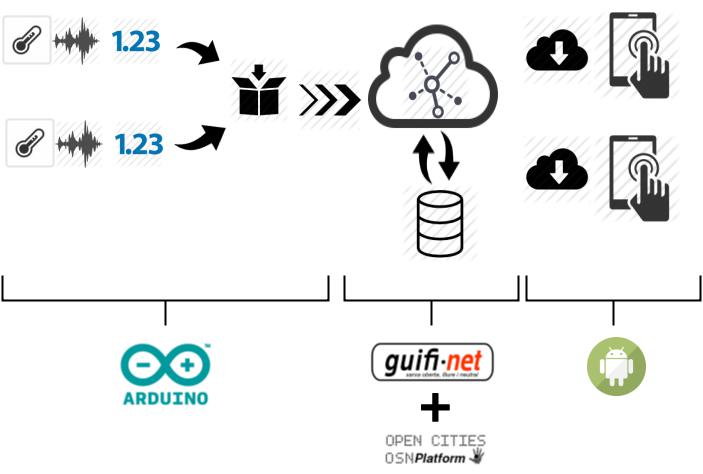
\includegraphics[scale=0.4]{../Final_Report/Figures/reportGeneralView.jpg} \end{center}
  }

\section{TECHNOLOGIES}

	\subsection{SENSORES}
	
		\begin{frame}
			\begin{columns}[t]
				\column{.5\textwidth}
				\centering
				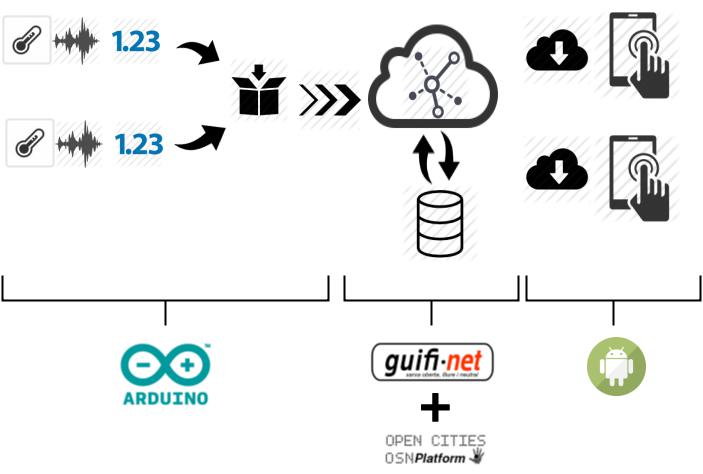
\includegraphics[width=5cm,height=3.5cm]{../Final_Report/Figures/reportGeneralView.jpg}\\
				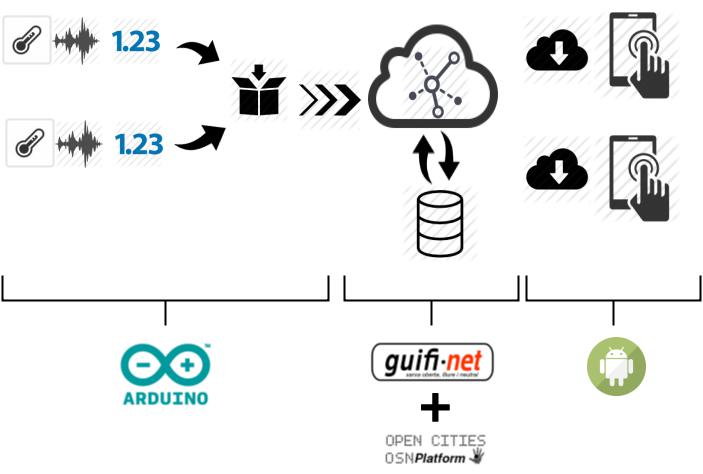
\includegraphics[width=5cm,height=4cm]{../Final_Report/Figures/reportGeneralView.jpg}
				\column{.5\textwidth}
				\centering
				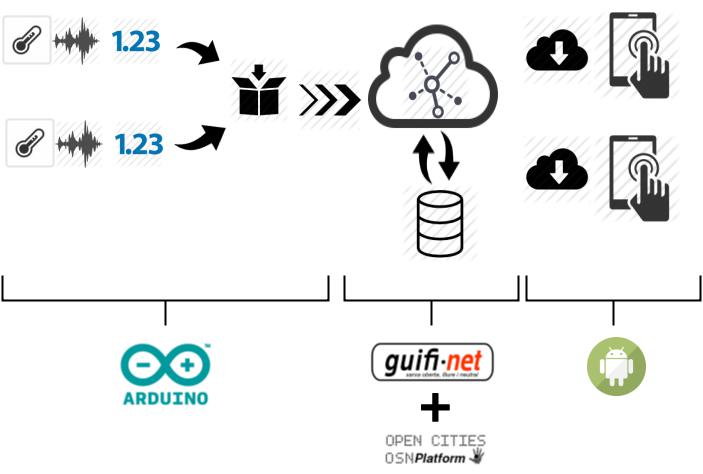
\includegraphics[width=5cm,height=4cm]{../Final_Report/Figures/reportGeneralView.jpg}\\
				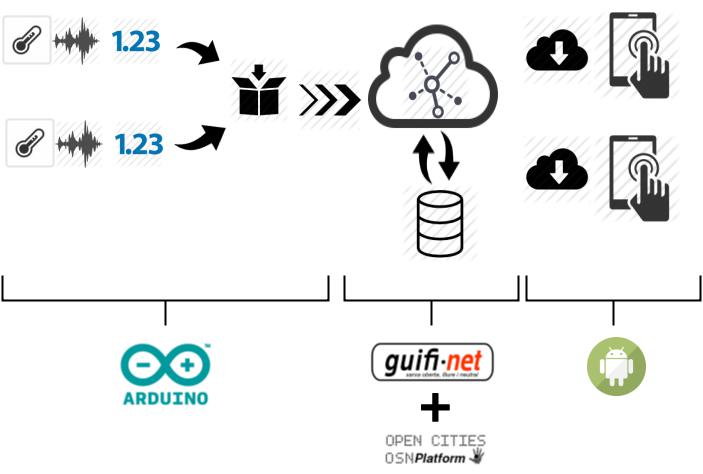
\includegraphics[width=5cm,height=4cm]{../Final_Report/Figures/reportGeneralView.jpg}
			\end{columns}
		\end{frame}
		
	\subsection{ARDUINO YUN + BRIDGE}
		HOLA
		
	\subsection{PYTHON + GEOJSON}
		HOLA
		
	\subsection{COMMUNITY NETWORK}
		HOLA
		
	\subsection{OPENCITIES}
		HOLA
		
	\subsection{ANDROID APP}
		HOLA
		

\section{TESTBED}
	HOLA
		
	
	\subsection{RESULTS}
		HOLA
		
	

\section{CONCLUSIONS}
	HOLA
		


\section{FUTURE WORK}
	HOLA
		

\section*{}
	\frame{
    \begin{center}
      \begin{huge}
      Thank you for your attention.
      \end{huge}
      \\
      \vspace{1cm}
      Reporsitory at github.com/SergioAlmendros/A-bottom-up-sensor-testbed	 \\ 
      \pause
      \vspace{1cm}
      \begin{huge}
      Any questions?
      \end{huge}
    \end{center}
	}


\end{document} 

















